\documentclass[pscyr]{hedlab}
\usepackage[russian]{babel}
\usepackage{graphicx}
\graphicspath{{images/}}
\usepackage{listings}

\lstset{
  basicstyle=\footnotesize,
  inputencoding=utf8,
  extendedchars=True,
  language=C,
  numbers=left,
  numberstyle=\footnotesize,
  breakatwhitespace=\false,
  breaklines=True,
  tabsize=2,
  keepspaces=true,
}

\labname{Разработка веб-приложения с использованием технологии ASP.NET}
\labnum{2}
\student{Голубев~А.~В., САПР-1.1п}
\labdate{}

\begin{document}

  \makeheader

  \emph{Цель:} получить практические навыки создания многостраничных
  веб-приложений и реализации обмена информацией между страницами.
  
  \emph{Задание:} разработайте прикладной веб-сайт, удовлетворяющий следующим
  требованиям. Он должен иметь:
  \begin{itemize}
    \item не менее пяти веб-форм, связанных между собой гиперссылками;
    \item не менее 10 элементов управления на каждой веб-странице, включая
      элементы ввода информации;
    \item не менее 5 методов обработки событий для каждой веб-страницы.
  \end{itemize}
  Реализовать механизм передачи информации между страницами с использованием
  переменной сессии.

  \emph{Выполнение лабораторной работы:}
  
  \textbf{Страница \#1:} опросник страница 1
  \begin{figure}[h!]
    \center
    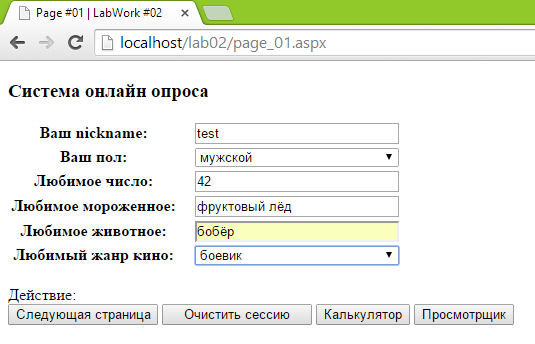
\includegraphics[width=.47\textwidth]{lab02_01}
  \end{figure}
  \lstinputlisting{./code/lab02_page_01.aspx.cs}
  
  \textbf{Страница \#2:} опросник страница 2
  \begin{figure}[h!]
    \center
    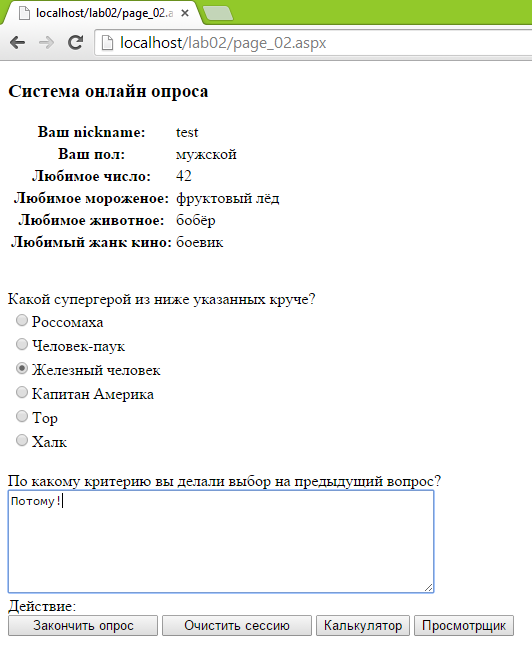
\includegraphics[width=.47\textwidth]{lab02_02}
  \end{figure}
  \lstinputlisting{./code/lab02_page_02.aspx.cs}
  
  \newpage
  
  \textbf{Страница \#3:} опросник результаты
  \begin{figure}[h!]
    \center
    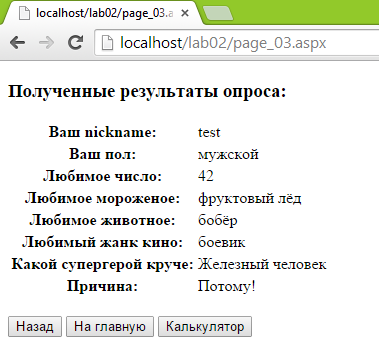
\includegraphics[width=.47\textwidth]{lab02_03}
  \end{figure}
  \lstinputlisting{./code/lab02_page_03.aspx.cs}
  
  \textbf{Страница \#4:} калькулятор
  \begin{figure}[h!]
    \center
    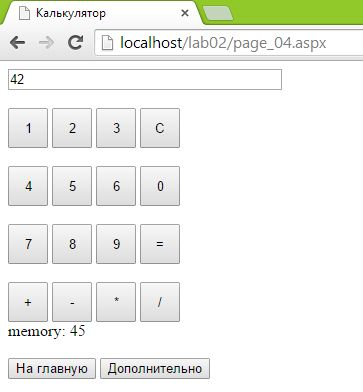
\includegraphics[width=.47\textwidth]{lab02_04}
  \end{figure}
  \lstinputlisting{./code/lab02_page_04.aspx.cs}
  
  \newpage
  
  \textbf{Страница \#5:} просмотрщик изображений
  \begin{figure}[h!]
    \center
    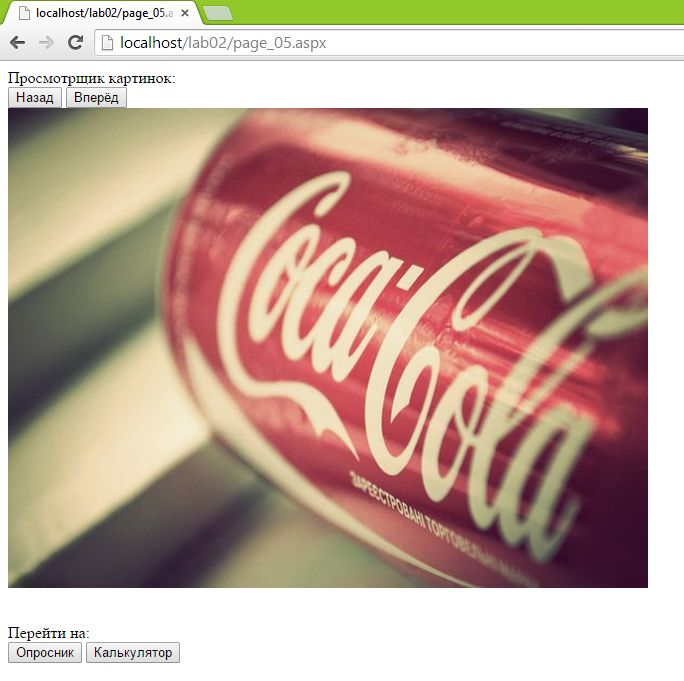
\includegraphics[width=.47\textwidth]{lab02_05}
  \end{figure}
  \lstinputlisting{./code/lab02_page_05.aspx.cs}
  
  \vspace{-1.5em}  
  \emph{Вывод:} в результате проделанной работы
  \vspace{-.5em}  
  \begin{enumerate}
    \itemsep -5pt
    \item установил и настроил веб-сервер Microsoft IIS;
    \item установил инструмент разработки веб-приложений Microsoft Visual
      Studio и СУБД Microsoft SQL Server;
    \item создал и запустил веб-узел.
  \end{enumerate}

\end{document}